\subsection{Memory and Bandwidth Overheads}
\label{s:eval:traces}
\label{sec:eval:traces}

%% The details of the on-chip cache
%% and backing store depend on the type traffic that passes through the switch.

In this section, we evaluate our key-value store design by running \TheSystem on
traces from both core Internet and data center switches to answer the following
questions:
\begin{CompactEnumerate}
\item What is a good size for the on-chip key value store?
\item How to equip the backing store to handle evictions?
\item How accurate are queries that aren't mergeable?
%%   What throughput should the backing store support?
%% \item What is the accuracy for queries not linear in state?
\end{CompactEnumerate}

\Para{Setup.}  We simulate a \TheSystem aggregation to count the number of
packets per \txtftuple over three separate {\em non-sampled} traces: two
five-minute traces from core Internet switches, one from Chicago
(\textasciitilde{}150 million packets) in April 2016~\cite{caida2016} and one
from San Jose (\textasciitilde{}189 million packets) in June
2014~\cite{caida2014}; and a 2.5 hour university datacenter trace
(\textasciitilde{}100 million packets) from 2010~\cite{bensonDC}. We refer to
these traces as Core16, Core14, and DC, respectively.

The aggregation key (a \txtftuple) requires 104 bits, and we assume a 24-bit
counter value, which totals 128 bits per entry in the key-value store. As
discussed in \Sec{hardware-feasibility}, our hardware design uses an 8-way LRU
cache. However, we also evaluate two other geometries: a hash table, which
evicts the incumbent key upon a collision, and a fully associative LRU
cache. Comparing our 8-way LRU with other hardware designs lets us evaluate the
tradeoff between hardware complexity, memory, accuracy, and eviction rate.

Based on an analysis of the traces, we use an average packet size of 700 bytes
and a network utilization of 30\%, to translate the number of evictions in our
results to an eviction rate (in packets per second) for a switch processing one
billion 64-byte packets per second.

\Para{On-chip cache size}.  The on-chip cache size significantly impacts the
eviction rate for mergeable queries, and the accuracy for queries that are not
mergeable. A larger cache causes fewer evictions---and hence a smaller load---on
the backing store. For non-mergeable aggregations, fewer evictions also produces
a higher accuracy. However, a larger cache size demands a larger silicon die
area and is more costly to manufacture.

Current SRAM densities are
$\approx7000\nicefrac{Kb}{mm^2}$~\cite{sram_estimate}, and the smallest
switching chips occupy 200 \si{\milli\metre\squared}~\cite{gibb_parsing}.
Therefore, a 32-Mbit cache in SRAM costs under 2.5\% additional area, which we believe is a reasonable overhead. Our trace-driven simulations thus target a 32-Mbit cache, while testing
a range from 8 Mbits ($2^{16}$ pairs) to 256 Mbits ($2^{21}$ pairs).

\Para{Eviction Rate.} Each key-value pair evicted from the switch must be streamed to a backing store.
This requires the backing store to be able to process packets at the eviction rate. We measure the eviction rates over (a) the 3 traces using the 8-way LRU geometry (\Fig{eviction-traces}) and (b) the three geometries for the DC trace (\Fig{eviction-geo}).
\begin{figure}[ht]
\centering
\vspace{-0.1in}
\begin{subfigure}[t]{0.48\columnwidth}
\raggedright
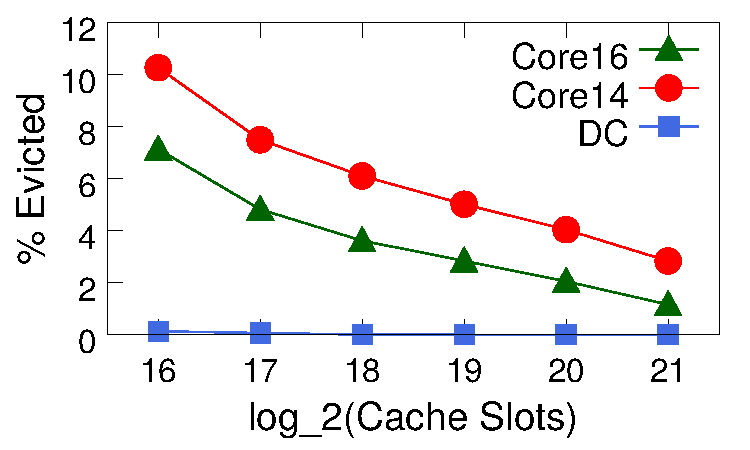
\includegraphics[width=\linewidth]{pq_eviction-rate-alltraces.pdf}
\caption{By trace}
\label{fig:eviction-traces}
\end{subfigure}
\begin{subfigure}[t]{0.48\columnwidth}
\raggedleft
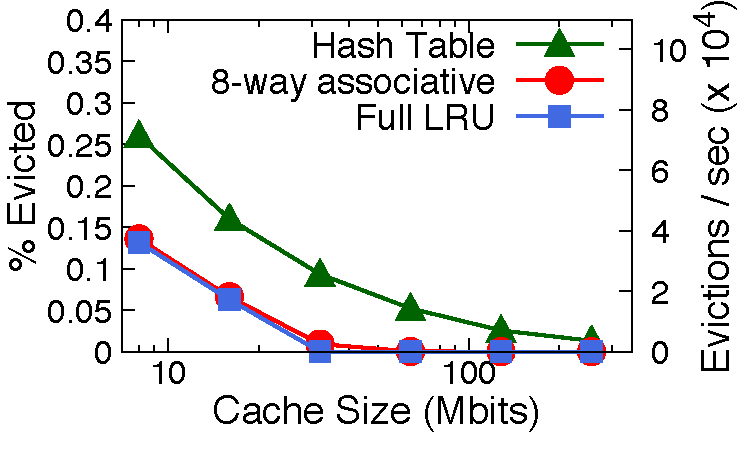
\includegraphics[width=\linewidth]{pq_eviction-rate-geo-dc.pdf}
\caption{By cache geometry (DC)}
\label{fig:eviction-geo}
\end{subfigure}
\caption{Measured eviction rates to the backing store.}
\end{figure}

The results offer three insights. First, a full LRU offers the lowest eviction
rates, since the entire LRU must be filled before an eviction occurs. However,
the 8-way associative cache comes within 2\% of this optimum, suggesting that it
is a good compromise: it avoids the hardware complexity of a full LRU without
compromising much on eviction rate. 
Second, the percentage of packets that result in an eviction at the target cache size of 32 Mbits is $\approx6\%$ for core internet switches. For the typical workload described above, this corresponds to an eviction rate of 1.67M packets per second. This is within the capabilities of multi-core scale-out key-value stores~\cite{redis_benchmark, memcached_benchmark, redis_vs_memcached, redis_vs_memcached_update}.
Third, the university datacenter setting, which is a target use case for Marple,
demands extremely little from the backing store since it has fewer unique keys
and thus fewer evictions, requiring it to sustain only 2500 packets per
second. A single processor core can handle this load. Additionally, a shorter
query that lasts only 5 minutes incurs only 3 evictions per second.

%TODO(vikram): fill in these numbers.
In context, the backing store requirements are modest. For a single ToR switch in a datacenter running at 640Gbps, a single 8-core server is sufficient to handle the eviction load. A multi-pipeline core router running at 6.4Tbps (\eg~\cite{tofino}) requires 10 such servers or 3 32-core machines. Note that the cost of these servers is low relative to the cost of the core router itself.

\Para{Accuracy of non-mergeable queries.}
Queries that are neither linear-in-state nor associative cannot be merged in the
backing store. If a key from such a query is evicted multiple times, \TheSystem
can no longer guarantee its correctness, and marks it as invalid. However, these
keys are still valid over a shorter time interval (until they are re-inserted in the
cache after an eviction). We quantify a query's accuracy as the fraction
of \emph{valid} keys over the query's lifetime. Figure~\ref{fig:accuracy-traces}
shows how query accuracy varies among the three traces, with the DC trace
near perfect since it has fewer unique keys, and hence, evictions.

If the query is run over a shorter time interval, its accuracy is typically higher, since the cache may not be full and a smaller fraction of keys are evicted. 
Figure~\ref{fig:accuracy-time} shows the tradeoff between query interval and accuracy for a variety of cache sizes and geometries using the Core16 trace.
Shortening the query from 5 minutes to 1 minute boosts accuracy by 10\%. Users running non-mergeable aggregations should consider running shorter queries to increase accuracy.

\begin{figure}[ht]
\centering
\vspace{-0.1in}
\begin{subfigure}[t]{0.48\columnwidth}
\raggedright
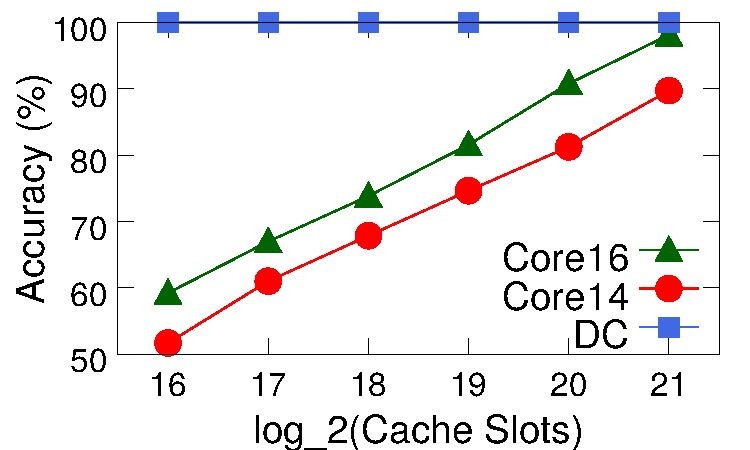
\includegraphics[width=\linewidth]{pq_accuracy-alltraces.pdf}
\caption{By trace}
\label{fig:accuracy-traces}
\end{subfigure}
\begin{subfigure}[t]{0.48\columnwidth}
\raggedleft
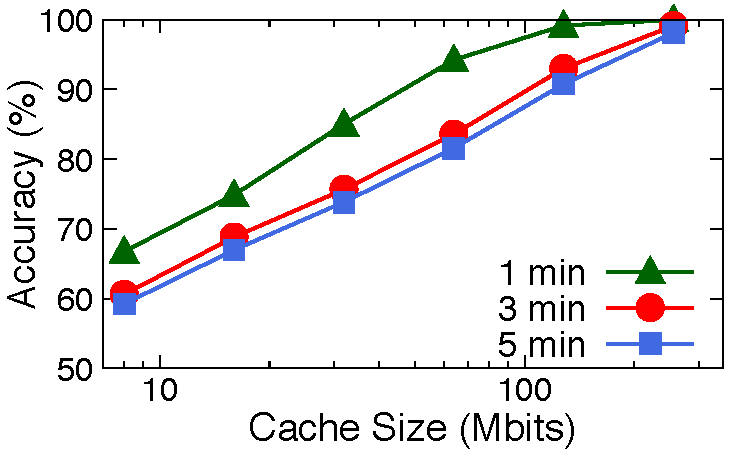
\includegraphics[width=\linewidth]{pq_accuracy-core-geo.pdf}
\caption{By cache geometry (Core16)}
\label{fig:accuracy-time}
\end{subfigure}
\caption{Query accuracy for non-mergeable aggregations.}
\end{figure}
